%%%%%%%%%%%%%%%%%%%%%%%%%%%%%%%%%%%%%%%%%
% Jacobs Portrait Poster
% LaTeX Template
% Version 1.0 (31/08/2015)
% (Based on Version 1.0 (29/03/13) of the landscape template
%
% Created by:
% Computational Physics and Biophysics Group, Jacobs University
% https://teamwork.jacobs-university.de:8443/confluence/display/CoPandBiG/LaTeX+Poster
% 
% Further modified by:
% Nathaniel Johnston (nathaniel@njohnston.ca)
%
% Portrait version by:
% John Hammersley
%
% The landscape version of this template was downloaded from:
% http://www.LaTeXTemplates.com
%
% License:
% CC BY-NC-SA 3.0 (http://creativecommons.org/licenses/by-nc-sa/3.0/)
%
%%%%%%%%%%%%%%%%%%%%%%%%%%%%%%%%%%%%%%%%%

%----------------------------------------------------------------------------------------
%	PACKAGES AND OTHER DOCUMENT CONFIGURATIONS
%----------------------------------------------------------------------------------------

\documentclass[final, english]{beamer}

\usepackage[size=a0, scale=1.24]{beamerposter} % Use the beamerposter package for laying out the poster

\usetheme{confposter} % Use the confposter theme supplied with this template

\setbeamercolor{block title}{fg=ngreen,bg=white} % Colors of the block titles
\setbeamercolor{block body}{fg=black,bg=white} % Colors of the body of blocks
\setbeamercolor{block alerted title}{fg=white,bg=dblue!70} % Colors of the highlighted block titles
\setbeamercolor{block alerted body}{fg=black,bg=dblue!10} % Colors of the body of highlighted blocks
% Many more colors are available for use in beamerthemeconfposter.sty


%-----------------------------------------------------------
% Define the column widths and overall poster size
% To set effective sepwid, onecolwid and twocolwid values, first choose how many columns you want and how much separation you want between columns
% In this template, the separation width chosen is 0.024 of the paper width and a 4-column layout
% onecolwid should therefore be (1-(# of columns+1)*sepwid)/# of columns e.g. (1-(4+1)*0.024)/4 = 0.22
% Set twocolwid to be (2*onecolwid)+sepwid = 0.464
% Set threecolwid to be (3*onecolwid)+2*sepwid = 0.708

\newlength{\sepwid}
\newlength{\onecolwid}
\newlength{\twocolwid}
\newlength{\threecolwid}
%\setlength{\paperwidth}{36in} % A0 width: 46.8in
%\setlength{\paperheight}{48in} % A0 height: 33.1in
\setlength{\sepwid}{0.024\paperwidth} % Separation width (white space) between columns
\setlength{\onecolwid}{0.22\paperwidth} % Width of one column
\setlength{\twocolwid}{0.464\paperwidth} % Width of two columns
\setlength{\threecolwid}{0.708\paperwidth} % Width of three columns
\setlength{\topmargin}{-0.5in} % Reduce the top margin size
%-----------------------------------------------------------

\usepackage{graphicx}  % Required for including images

\usepackage{multicol}
%\usepackage{booktabs} % Top and bottom rules for tables

%----------------------------------------------------------------------------------------
%	TITLE SECTION 
%----------------------------------------------------------------------------------------

\title{Joint Optimization of a Reserved Lane with an Infinite Passenger Demand} % Poster title

\author{Martin Briand (Feb 2025), \href{mailto:martin.briand@enpc.fr}{martin.briand@enpc.fr}} % Author(s)

\institute{LVMT, École Nationale des Ponts et Chaussées} % Institution(s)

%----------------------------------------------------------------------------------------

\begin{document}

\addtobeamertemplate{block end}{}{\vspace*{2ex}} % White space under blocks
\addtobeamertemplate{block alerted end}{}{\vspace*{2ex}} % White space under highlighted (alert) blocks

\setlength{\belowcaptionskip}{2ex} % White space under figures
\setlength\belowdisplayshortskip{2ex} % White space under equations

\begin{frame}[t] % The whole poster is enclosed in one beamer frame

\begin{columns}[t] % The whole poster consists of three major columns, the second of which is split into two columns twice - the [t] option aligns each column's content to the top

\begin{column}{\sepwid}\end{column} % Empty spacer column

\begin{column}{\twocolwid} % The first column

\begin{block}{Introduction}

In France, the Trapeze project aims to bridge the gap between having a not always efficient reserved High Occupancy Vehicle (HOV) and having no reserved lane at all.

\bigskip

Rather than authorizing drivers to pay for using the reserved capacity while solo driving (often seen as politically infeasible), drivers on the reserved lane have a reduced utility by being enforced to carry any passenger waiting at some carpool stations, if any \cite{vinci_autoroutes_experimentation_nodate}.

\end{block}

\begin{figure}
    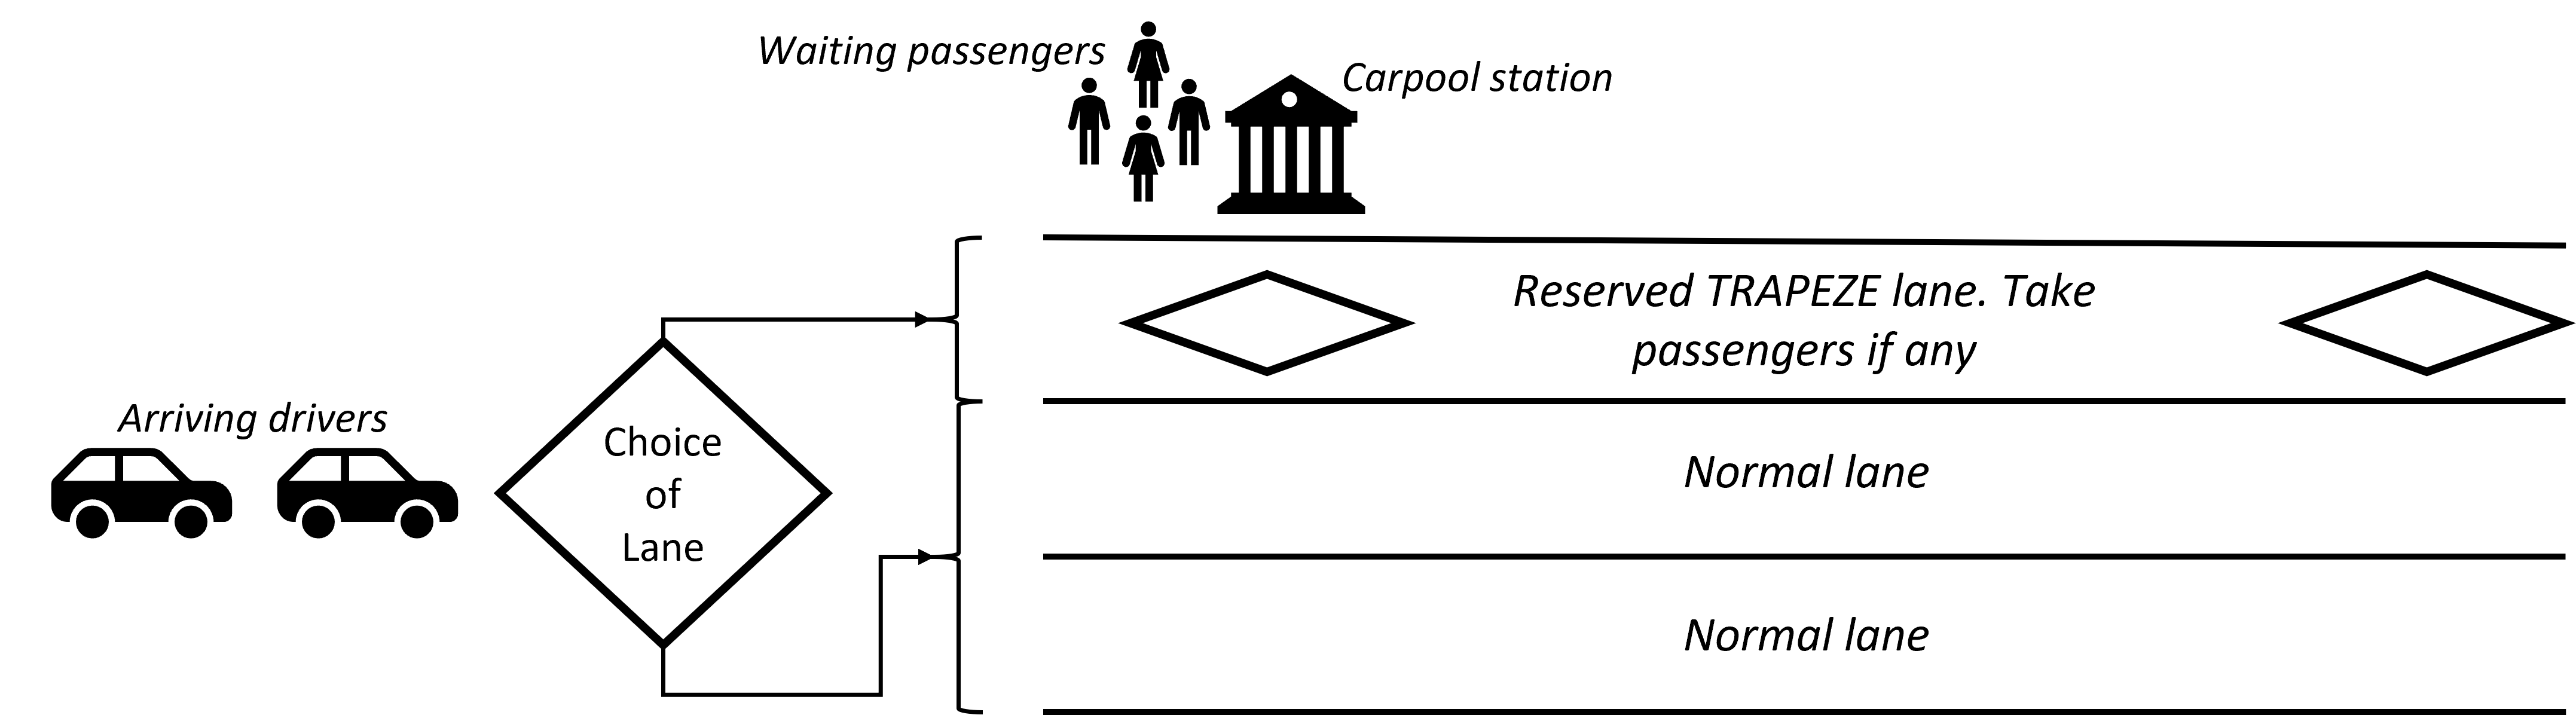
\includegraphics[width=\linewidth]{figures/schema_trapeze_system.png}
    \caption{Schema of the trapeze framework}
\end{figure}

\begin{alertblock}{Objectives}
\begin{itemize}
    \item Understand how such a system could behave and find ways to obtain social optima.
    \item Test this behavior with many distributions of users
\end{itemize}

\end{alertblock}

\begin{block}{Hypotheses and notations}
    \begin{itemize}
        \item For the sake of simplicity (this will change later), passenger demand is supposed exogenous and infinite.
        \item For the sake of simplicity (this will change later), all drivers are supposed identical.
        \item A fixed number $N$ of drivers are allowed to choose between:
        \begin{itemize}
            \item $N_d$ drivers proposing to share their drive on the reserved capacity with passengers. Additional to congestion costs and car usage cost, they incur an inconvenience cost $\Delta$.
            \item $N_s$ drivers not sharing their drive on traveling on the regular lanes.
        \end{itemize}
        \item All drivers have classical bottleneck time cost structures $0 < \beta < \alpha$, $0 < \gamma$ and $t^*$ where:
        \begin{itemize}
            \item $\beta$ is travel time opportunity cost;
            \item $\alpha$ is the early delay opportunity cost;
            \item $\gamma$ is the late delay opportunity cost;
            \item $t^*$ is the desired arrival time.
        \end{itemize}
        \item The road has a capacity $s$ which is split between reserved capacity $\varphi s$ and normal capacity $( 1-\varphi ) s$, with$0 \leq \varphi \leq 1$.
        \item A Trapeze operator can charge drivers on the reserved lane a given varying toll price $\rho (t)$ which can potentially negative.
    \end{itemize}
\end{block}

\begin{alertblock}{Theorem (1/2)}

    For a fixed $\varphi$, for any function $\rho (t)$ that minimizes social cost there exists a $\rho_0$ such that $\rho ' (t) = \rho_0 + \rho^*(t)$ is also social cost minimizing, where:

    \begin{equation*}
        \begin{array}{ll}
        \rho^*(t) = \left\{
            \begin{array}{ll}
                0 & \text{if } t<t^0\\
                \delta \frac{N}{s} - \beta (t^* - t) & \text{if } t\in [t^0, t^*]\\
                \delta \frac{N}{s} - \gamma (t-t^*) & \text{if } t \in [t^*, t^1]\\
                0 & \text{if } t>t^1
        \end{array}
        \right.
        & \text{with }\left\{
            \begin{array}{l}
                t^0 = t^* - \frac{\gamma}{\beta + \gamma} \cdot \frac{N_d}{\varphi s}\\
                t^1 = t^* + \frac{\beta}{\beta + \gamma} \cdot \frac{N_d}{\varphi s}
            \end{array}
            \right.
    \end{array}
    \end{equation*}
    
    Among the optimal tolls of these forms, there is always one that can raise a non-negative profit.

\end{alertblock}
    

\end{column} % End of the first column

\begin{column}{\sepwid}\end{column} % Empty spacer column

\begin{column}{\twocolwid} % Begin a column which is two columns wide (column 2)

\begin{alertblock}{Theorem (2/2)}

    Similarly, allowing $\varphi$ to vary or not, for any $(\varphi, \rho (t))$ that minimizes social cost, there exists a $\rho_0$ such that $\varphi, \rho ' (t)$ is also a social cost minimizing toll.

    Again, at least one of the optimal toll can raise a non-negative profit.

\end{alertblock} 

\begin{block}{Results}

    Only allowing the toll to vary for a fixed value of $\varphi$, Figure \ref{figure_fixed_phi} shows that it is likely the case that the optimal split will be optimal. The road usage is the most intensive whatever the value of $\varphi$ when the ratio of costs $\left. \Delta \middle/ \frac{\delta N}{s} \right.$ is close to one.

    \begin{figure}
        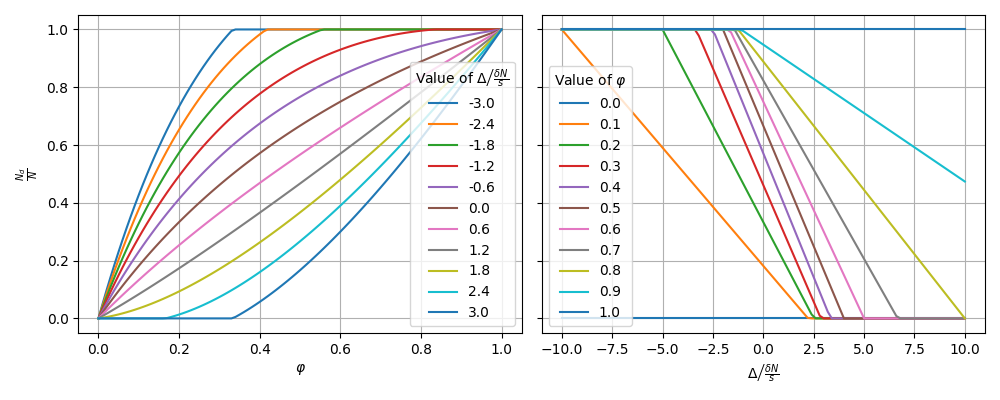
\includegraphics[width=\linewidth]{figures/fixed_phi.png}
        \caption{Value}
        \label{figure_fixed_phi}
    \end{figure}

    Allowing the road capacity split and the toll to be optimized jointly, it now appears that it is useful to reserve some of the road capacity iif $\sqrt{2} - 1 < \left. \Delta \middle/ \frac{\delta N}{s} \right. < 2 - \sqrt{2}$ (see Figure \ref{figure_varying_phi}).

    \begin{figure}
        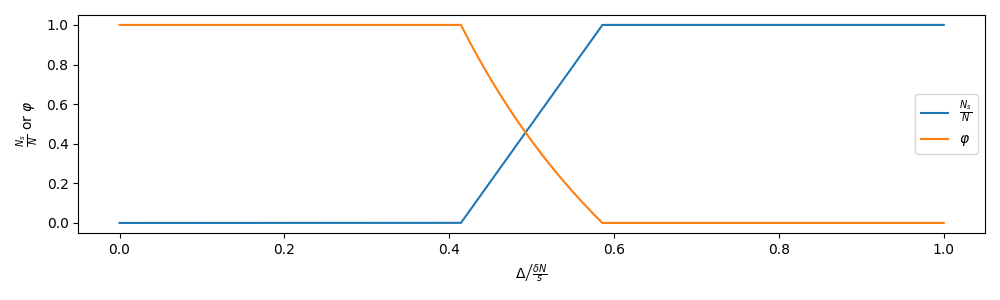
\includegraphics[width=\linewidth]{figures/varying_phi.png}
        \caption{Figure caption}
        \label{figure_varying_phi}
    \end{figure}
\end{block}

\begin{block}{Conclusion and limits}
    While for a fixed share of reserved capacity, an optimal toll will achieve a usage of both lanes, the interior solution interval is much smaller when allowing the reserved capacity to be jointly optimized. An amplification phenomenon takes place: more reserved capacity implies more carpooler implies more reserved capacity until full capacity.

    \bigskip

    Some limits should be stressed though: 1. passengers could be endogenous, 2. and variability of $\Delta$ between travelers should be allowed.
\end{block}


\begin{block}{References}

    \begin{multicols}{2}
        \nocite{*} % Insert publications even if they are not cited in the poster
        \footnotesize{\bibliographystyle{unsrt}
        \bibliography{Poster_steve}\vspace{0.75in}}
	\end{multicols}
    
    
        
\end{block}


\end{column} % End of the second column

\begin{column}{\sepwid}\end{column} % Empty spacer column


\end{columns} % End of all the columns in the poster

\tikz[remember picture, overlay]
    \path (current page.north east) ++ (-11.5,-13) node {
\includegraphics[scale=0.6]{figures/LVMT_logo.png}};

\tikz[remember picture, overlay]
    \path (current page.north west) ++ (12,-13) node {
\includegraphics[scale=0.65]{figures/ENPC_logo.png}};



\end{frame} % End of the enclosing frame



\end{document}
